\documentclass{sig-alternate}
\usepackage{amsmath}
\usepackage{amssymb}
\usepackage{array}
\usepackage{bm}
\usepackage{booktabs}
\usepackage{caption}
\usepackage{enumitem}
\usepackage{graphicx}
\usepackage{mathtools}
\usepackage{multirow}
\usepackage{subcaption}
\usepackage{tabularx}
\usepackage{verbatim}
\usepackage{colortbl}
\usepackage[table]{xcolor}

\newcommand\rankeq{\mathrel{\overset{\makebox[0pt]{\mbox{\normalfont\tiny\sffamily rank}}}{=}}}
\newcommand{\bigcell}[2]{\begin{tabular}{@{}#1@{}}#2\end{tabular}}

\setlist[itemize]{noitemsep}  % remove space between list items
\setlist[enumerate]{noitemsep}  % remove space between list items

\begin{document}

\author{[Blind]}

\title{Pseudo-Relevance Query Performance Prediction for Information Retrieval}

\maketitle
\begin{abstract}
Techniques for estimating the effectiveness of an information retrieval system in the absence of relevance judgments, known as query performance prediction (QPP), generally work by associating some property of a query or its document result set with an evaluation metric like mean average precision. We propose a method of QPP that directly incorporates notions of relevance into the prediction process. To do this, we rely on the well-known information retrieval technique of pseudo-relevance feedback to approximate relevance judgments and to reformulate the query. Our experiments indicate that this approach is very effective at predicting query performance.
\end{abstract}

\section{Introduction}\label{section.intro}

Query performance prediction (QPP) is the task of estimating, without reference to relevance judgments, the success of an information retrieval (IR) system in retrieving results for a submitted query. Prediction strategies generally use properties of the query or of the retrieved document set to quantify the success of a system. The former is called pre-retrieval prediction, while the latter is called post-retrieval prediction. On the whole, post-retrieval prediction outperforms pre-retrieval prediction, and our predictor belongs to this class.

In general, post-retrieval prediction methods tend to associate some property of the result set with the relevance of the result set in general (or, more accurately, some measurement thereof). These properties are usually intuitively suggestive of some form of stability or robustness, as discussed in Section \ref{section.related}. 

In this work, we propose a predictor inspired by pseudo-relevance feedback techniques that directly incorporates relevance metrics in the prediction process. We accomplish this by asserting that the top retreived documents in a ranked list for a query are relevant to that query; we then use these pseudo-relevance judgments to estimate document retrieval evaluation using natural variations on the query derived from the top ranked documents. 

\section{Related Work}\label{section.related}

A great deal of research has focused on QPP \cite{Carmel2010}. The most famous predictor is query clarity (QC) \cite{Cronen-Townsend2002}. Clarity is simply the KL-divergence of an expanded query language model and the collection as a whole:

\begin{flalign}\label{eq.clarity}
clarity(Q) = \sum_{w \in V} P(w|Q) \log \frac{P(w|Q)}{P(w|C)}
\end{flalign}

\noindent where $w$ is a term in the vocabulary $V$, $P(w|C)$ is the maximum likelihood estimate of $w$ in collection $C$, and $P(w|Q)$ is the probability of $w$ as computed by a relevance model \cite{Lavrenko2001}. 

%The latter are computed by

% \begin{flalign}\label{eq.rm}
% \sum_{D \in C} P(w|D) P(Q|D).
% \end{flalign}
% 
% \noindent $P(Q|D)$ is computed as in Eq. 

The idea underlying clarity is that a query whose top ranked documents are linguistically distinct from a generic background language model has likely done a better job identifying relevant documents than one whose top ranked documents resemble the background model. Several modifications of query clarity have been proposed, e.g. \cite{Diaz2004, Hauff2008, He2004}. We incorporate traditional query clarity as a baseline in our work.

One class of query performance predictor that is related to our work is query perturbation \cite{Vinay2006, Yom-Tov2005, Zhou2007}. These methods alter the query and measure the similarity of the results list across query variations; if the result list remains relatively constant, the system is believed to have little difficulty with the query. Our proposed method is fundamentally a form of query perturbation, with the alternative query forms derived from feedback documents.

Zhou \& Croft's query feedback (QF) method is a query perturbation predictor that holds some resemblance to our own \cite{Zhou2007}. Their method begins by constructing a new query from the top ranked documents. First, QF issues $Q$ against collection $C$, retrieving a results list $L$. By ranking each term $w$ in $L$ according to its contribution to query clarity (that is, its contribution to the KL-divergence with the collection) and selecting the top ranked terms, a new query $Q'$ is constructed. After retrieving results list $L'$ for $Q'$, the percentage overlap between $L$ and $L'$ is computed. This overlap is the QF score. Like our proposed method, the top ranked results give rise to alternate queries, and the results lists of the original and alternate queries are compared. Unlike ours, however, QF produces only a single alternate query; our method also differs in its scoring component, which directly models retrieval performance rather than simply measuring overlap as QF does. Because of its similarity to our method, we use query feedback as a second baseline.

\section{Pseudo-Relevance Performance Predictor}\label{section.method}

\subsection{Underlying Retrieval Model}\label{section.method.underlying}

Although our query performance predictor does not require it, in this paper we employ the standard multinomial query likelihood (QL) retrieval model to rank the relevance of a document $D$ to query $Q$.  Assuming a uniform distribution over documents, QL scores $D$ by the following:

\begin{flalign}\label{eq.ql}
P(Q|D) = \prod_{i=1}^{|Q|} P(q_i|\theta_D)
\end{flalign}

\noindent where $q_i$ is a word in $Q$ and $P(q_i|\theta_D)$ is estimated using Dirichlet smoothing:

\begin{flalign}\label{eq.dirichlet}
P(q_i|\theta_D) = \frac{c(q_i,D) + \mu \hat{P}(q_i|C)}{|D| + \mu}
\end{flalign}

\noindent where $c(q_i,D)$ is the frequency of $q_i$ in $D$, $|D|$ is the length of the document, $\hat{P}(q_i|C)$ is the maximum likelihood estimate of $q_i$ in collection $C$, and $\mu$ is a parameter. We set $\mu = 2500$ for all runs.

\subsection{Predicting Query Performance}\label{section.method.predicting}

\begin{figure*}
%\centering
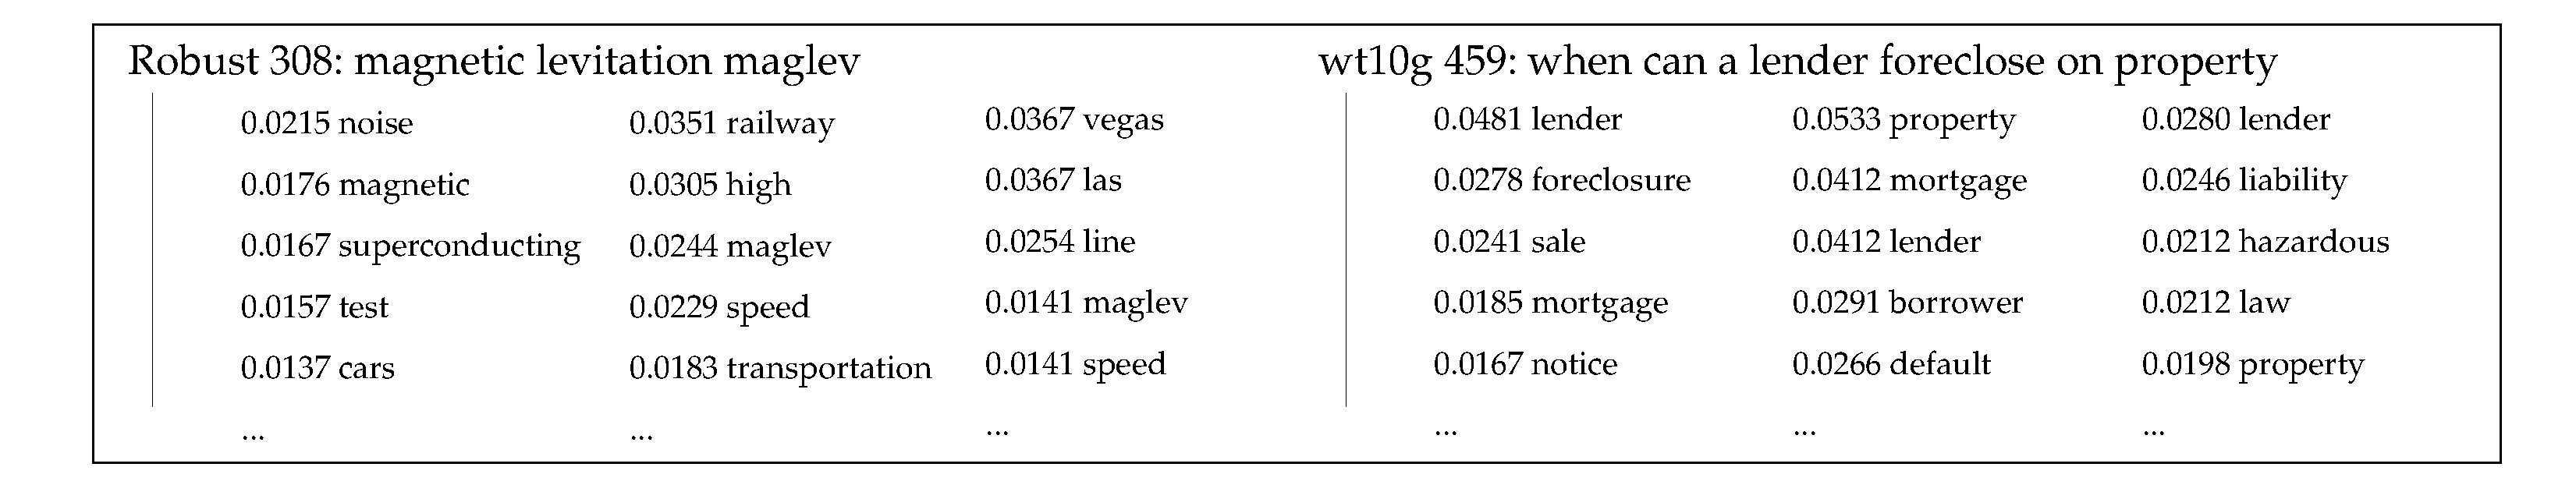
\includegraphics[width=\linewidth]{figures/example-queries.pdf}
\caption{Example pseudo-queries formed in our process. Each column displays the top five terms in the pseudo-query and their weights. The two original queries appear above ther respective pseudo-queries.}
\label{figure.queries}
\end{figure*}

Our query performance predictor, which we call the pseudo-evaluation performance predictor (PEval), is inspired by the pseudo-relevance feedback technique of treating the top ranked documents as relevant to the query. Doing so allows us to directly model the robustness of relevance metrics to query perturbation. We present the steps involved in our technique, followed by an explanation of key points:

\begin{enumerate}
	\item Issue query $Q$ against performance collection $C_p$; call the results list $R_p$
	\item Record the top $r$ documents in $R_p$ as relevant using each document's normalized retrieval score as the degree of relevance; all other documents are assumed to be non-relevant
	\item If $C_p \neq C_t$, issue $Q$ against target collection $C_t$; call the results list $R_t$
	\item For each document $D$ in $R_t$,
	\begin{enumerate}
		\item Construct a pseudo-query $Q_D$ consisting of the top $|Q_D|$ non-stop terms\footnote{We remove terms in the standard Indri stoplist: http://www.lemurproject.org/stopwords/stoplist.dft} in $D$
		\item Issue $Q_D$ against $C_p$; call the results list $R_{Q_D}$
		\item Score $R_{Q_D}$ for some relevance metric, e.g. average precision, using the pseudo-relevance judgments from Step 2.
	\end{enumerate}
	\item Average the scores computed in Step 4 to compute a single score for $Q$
\end{enumerate}

Essentially, our approach emulates an ad-hoc document retrieval evaluation using information from the true, original retrieval: we evaluate the ranked retrieval $R_{Q_D}$ for each query $Q_D$ using relevance judgments $R_p$.

Our model makes no assertions about the identity of the performance collection $C_p$. While it is valid to use the target collection as the performance collection, we hypothesize that the use of an external collection may yield better results. We investigate this idea in Section \ref{section.results.external}.

Both $r$ and $|Q_D|$ are free parameters in our approach, as are two additional parameters: $k$ controls the length of $R_t$, while $n$ controls the length of $R_{Q_D}$. In general, all parameters should be set empirically. Although not required mathematically, we only allow values of $n$ where $n \leq r$ since setting $n$ greater than $r$ prevents us from achieving perfect recall, i.e. from retrieving all pseudo-relevant documents.

One advantage to our model is the ability to predict specific retrieval metrics by estimating levels of relevance. As Step 2 states, we estimate levels of relevance by normalizing the retrieval scores of the documents in $R_p$. This follows from the pseudo-relevance feedback technique of treating top ranked documents as relevant by simply treating \textit{more highly} ranked documents as \textit{more relevant}. We use the normalized retrieval scores rather than the rankings themselves in order to allow documents to achieve similar levels of relevance if their scores are similar.

Because these relevance levels are normalized probabilities, they consist of continuous values (in contrast to TREC qrels which contain binary or discrete relevance grades), but are still valid for metrics that incorporate graded relevance judgments like normalized discounted cumulative gain (nDCG). Metrics that use only binary relevance metrics, like mean average precision (MAP), follow the typical procedure of treating all judgments greater than zero as relevant.

\section{Evaluation}\label{section.evaluation}

\subsection{Data}\label{section.evaluation.data}

We evaluate our procedure using a variety of TREC datasets that represent a variety of corpora properties:

\begin{itemize}
	\item AP newsire with topics 101-200 from TREC disks 1 and 2
	\item Robust with the 2004 topics from TREC disks 4 and 5
	\item wt10g with the topics 451-500 from the 2000 and 2001 TREC Web tracks
\end{itemize}

We also make use of an indexed dump of Wikipedia\footnote{http://en.wikipedia.org} as an external collection in some experiments.

\subsection{Parameters}\label{section.evaluation.runs}

Our predictor requires the setting of several parameters. We set $r$, $k$, and $n$ by cross-validation: we sweep over each parameter at the values $\{1, 5, 10, 20, 50, 75, 100\}$. As noted in Section \ref{section.method}, $n$ is only swept at values $\leq r$. We fix $|Q_D| = 20$ for all runs since using the entire length of $D$, $|D|$, is excessively expensive during retrieval.

For each run, we split the query set into two equal sized folds and run 2-fold cross-validation, using the train fold to determine the optimal parameter settings to apply to the test fold. We choose an equal split over other forms of cross-validation in order to provide a relatively large number of queries to each fold, leading to more stable correlation values. We repeat this procedure 100 times, splitting the query set randomly each time, and average the correlation values to compute an average query performance prediction score.

We perform the same procedure on the parameters involved in our baseline predictors. Query clarity requires a single parameter: the number of feedback documents; we sweep over the values $\{10, 50, 100, 250, 500, 750, 1000\}$ for this parameter. Query feedback has two parameters: the number of top ranked documents in results lists $L$ and $L'$, for which we consider values of $\{10, 20, 50, 75, 100, 500\}$, and the number of terms included in the newly formed query $Q'$, for which we consider $\{3, 5, 10, 15, 20\}$.

\section{Results}\label{section.results}

\begin{table}[t]
\centering
\begin{tabular}{|l|l|l|l|l|l|} \hline
& & \multicolumn{2}{c|}{MAP} & \multicolumn{2}{c|}{nDCG@20} \\ \cline{3-6}
Corpus & Run & Valid. & Max. & Valid. & Max \\ \hline\hline
\multirow{3}{*}{AP} & QC & 0.3933 & 0.5742 & 0.1858 & 0.3487 \\ \cline{2-6}
& QF & 0.3561 & 0.5637 & 0.2386 & 0.4467 \\ \cline{2-6}
%& PEval-flip & 0.3518 & 0.5661 & \textbf{0.2805} & \textbf{0.5092} \\ \cline{2-6}
& PEval & \textbf{0.4152}$^{cf}$ & \textbf{0.6115} & \textbf{0.2513}$^{c}$ & \textbf{0.4880} \\ \hline\hline
\multirow{3}{*}{wt10g} & QC & 0.1054 & 0.2226 & 0.0027 & 0.0674* \\ \cline{2-6}
& QF & 0.2220 & 0.3847 & 0.1775 & 0.3613 \\ \cline{2-6}
%& PEval-flip & 0.2687 & \textbf{0.4665} & 0.1961 & 0.3949 \\ \cline{2-6}
& PEval & \textbf{0.2912}$^{cf}$ & \textbf{0.4615} & \textbf{0.1965}$^{c}$ & \textbf{0.4173} \\ \hline\hline
\multirow{3}{*}{Robust} & QC & 0.2942 & 0.4284 & 0.2292 & 0.3165 \\ \cline{2-6}
& QF & 0.3544 & 0.5073 & \textbf{0.3347} & 0.4926 \\ \cline{2-6}
%& PEval-flip & 0.3973 & 0.5743 & \textbf{0.3410} & \textbf{0.5094} \\ \cline{2-6}
& PEval & \textbf{0.3985}$^{cf}$ & \textbf{0.5791} & 0.3297$^{c}$ & \textbf{0.5047} \\ \hline
\end{tabular}
\caption{Cross-validated and maximum Pearson's $r$ correlation of predictors for each collection. $^c$ and $^f$ indicate statistically significant improvement at $p < 0.05$ over query clarity and query feedback respectively. Bolded values are the largest observed per corpus/metric summary. All correlations are statistically significant unless marked with an asterisk (*).}
\label{table.results.self.pearson}
\end{table}

\begin{table}[t]
\centering
\begin{tabular}{|l|l|l|l|l|l|} \hline
& & \multicolumn{2}{c|}{MAP} & \multicolumn{2}{c|}{nDCG@20} \\ \cline{3-6}
Corpus & Run & Valid. & Max. & Valid. & Max. \\ \hline\hline
\multirow{3}{*}{AP} & QC & 0.3965 & 0.4157 & 0.1997 & 0.2276 \\ \cline{2-6}
& QF & 0.3601 & 0.4215 & 0.2381 & 0.3010 \\ \cline{2-6}
%& PEval-flip & 0.4129 & 0.4670 & \textbf{0.2757} & \textbf{0.3543} \\ \cline{2-6}
& PEval & \textbf{0.4554}$^{cf}$ & \textbf{0.4962} & \textbf{0.2521}$^{c}$ & \textbf{0.3378} \\ \hline\hline
\multirow{3}{*}{wt10g} & QC & 0.0779 & 0.1221* & -0.0017 & 0.0262*\\ \cline{2-6}
& QF & 0.2088 & 0.2843 & 0.1529 & 0.2411 \\ \cline{2-6}
%& PEval-flip & \textbf{0.3020} & \textbf{0.3772} & 0.1960 & 0.2844\\ \cline{2-6}
& PEval & \textbf{0.2734}$^{cf}$ & \textbf{0.3642} & \textbf{0.2207}$^{cf}$ & \textbf{0.3053} \\ \hline\hline
\multirow{3}{*}{Robust} & QC & 0.3070 & 0.3159 & 0.2357 & 0.2418 \\ \cline{2-6}
& QF & 0.3508 & 0.3745 & 0.3347 & \textbf{0.3646} \\ \cline{2-6}
%& PEval-flip & 0.4029 & 0.4148 & 0.3410 & \textbf{0.3698} \\ \cline{2-6}
& PEval & \textbf{0.4129}$^{cf}$ & \textbf{0.4273} & \textbf{0.3442}$^{cf}$ & 0.3634 \\ \hline
\end{tabular}
\caption{Cross-validated and maximum Kendall's $\tau$ correlation of predictors for each collection. $^c$ and $^f$ indicate statistically significant improvement at $p < 0.05$ over query clarity and query feedback respectively. Bolded values are the largest observed per corpus/metric summary. All correlations are statistically significant unless marked with an asterisk (*).}
\label{table.results.self.kendall}
\end{table}

A few sample pseudo-queries are shown in Figure \ref{figure.queries} along with the original query that they are meant to approximate. We can see that in general the pseudo-queries tend to stay related to the topic expressed in the original query; in some cases, however, such as the final pseudo-query shown for the original robust query, a great deal of noise can be introduced. This type of noise arises naturally from the language of the retrieved documents.

The results of our predictor as well as the two baselines are shown in Tables \ref{table.results.self.pearson} and \ref{table.results.self.kendall}; the former displays Pearson's $r$ correlation with the target metric (MAP or nDCG@20) while the latter displays Kendall's $\tau$ rank correlation.

We report the average of the cross-validated runs in the "Valid." column. Values marked with superscripts indicate statistically significant improvement over baselines at $p < 0.05$ using a one-tailed paired t-test. The tables show that PEval outperforms the baselines whenever MAP is the target metric; it also outperforms QC with nDCG@20 as the target metric in all cases and outperforms QF for wt10g and robust with Kendall's $\tau$ correlation.

We also report the maximum correlation value seen across all parameter settings. This is an oracle metric in that it uses the full set of queries and therefore the full set of relevance judgments. As can be seen in Tables \ref{table.results.self.pearson} and \ref{table.results.self.kendall}, the maximum prediction accuracy of PEval is usually the highest across predictors and is often much higher than either baseline. The maximum value is included because it is suggestive of the potential of each predictor.

\subsection{Using External Corpora for Prediction}\label{section.results.external}

\begin{table}
\centering
\begin{tabular}{|l|l|l|l|l|l|} \hline
& \multicolumn{2}{c|}{MAP} & \multicolumn{2}{c|}{nDCG@20} \\ \cline{2-5}
Corpus & Valid. & Max. & Valid. & Max. \\ \hline\hline
% \multirow{2}{*}{AP} & QC$_w$ & 0.1938$^{\downarrow}$ & & 0.0873$^{\downarrow}$ & \\ \hline
AP & \textbf{0.4495}$^{\uparrow}$ & \textbf{0.6740} & \textbf{0.3593}$^{\uparrow}$ & \textbf{0.5742} \\ \hline
% \multirow{2}{*}{wt10g} & QC$_w$ & 0.1496$^{\uparrow}$ & & 0.0996$^{\uparrow}$ & \\ \hline
wt10g & \textbf{0.3344}$^{\uparrow}$ & \textbf{0.5487} & \textbf{0.2851}$^{\uparrow}$ & \textbf{0.5163} \\ \hline
% \multirow{2}{*}{Robust} & QC$_w$ & 0.2359$^{\downarrow}$ & & 0.2078$^{\downarrow}$ & \\ \hline
Robust & 0.3778$^{\downarrow}$ & 0.4821 & 0.2984$^{\downarrow}$ & 0.4333 \\ \hline
\end{tabular}
\caption{Pearson's $r$ correlation for PEval using Wikipedia as the performance collection. $\uparrow$ and $\downarrow$ indicate statistically significant ($p < 0.05$) improvement and decline, respectively, relative to the corresponding run in Table \ref{table.results.self.pearson}. Bolded values are greater than than the corresponding value in Table \ref{table.results.self.pearson}.}
\label{table.results.wiki.pearson}
\end{table}

\begin{table}
\centering
\begin{tabular}{|l|l|l|l|l|l|} \hline
& \multicolumn{2}{c|}{MAP} & \multicolumn{2}{c|}{nDCG@20} \\ \cline{2-5}
Corpus & Valid. & Max. & Valid. & Max. \\ \hline\hline
% \multirow{2}{*}{AP} & QC$_w$ & 0.1872$^{\downarrow}$ & & 0.0924$^{\downarrow}$ & \\ \hline
AP & \textbf{0.4693}$^{\uparrow}$ & \textbf{0.5082} & \textbf{0.3589}$^{\uparrow}$ & \textbf{0.4170} \\ \hline
% \multirow{2}{*}{wt10g} & QC$_w$ & 0.1538$^{\uparrow}$ & & 0.1028$^{\uparrow}$ & \\ \hline
wt10g & \textbf{0.3272}$^{\uparrow}$ & \textbf{0.4131} & \textbf{0.2845}$^{\uparrow}$ & \textbf{0.3781} \\ \hline
% \multirow{2}{*}{Robust} & QC$_w$ & 0.2295$^{\downarrow}$ & & 0.2001$^{\downarrow}$ & \\ \hline
Robust & 0.3693$^{\downarrow}$ & 0.3909 & 0.3040$^{\downarrow}$ & 0.3355 \\ \hline
\end{tabular}
\caption{Kendall's $\tau$ correlation for PEval using Wikipedia as the performance collection. $\uparrow$ and $\downarrow$ indicate statistically significant ($p < 0.05$) improvement and decline, respectively, relative to the corresponding run in Table \ref{table.results.self.kendall}. Bolded values are greater than than the corresponding value in Table \ref{table.results.self.kendall}.}
\label{table.results.wiki.kendall}
\end{table}

As mentioned in Section \ref{section.method.predicting}, PEval does not require that the performance collection and target collection be the same. One intuitive reason an external collection may be beneficial is if the top ranked documents $R_t$ are not representative of the true relevant documents in the collection; in this case, we would expect PEval to overpredict performance since the evaluation of the pseudo-queries based on $R_t$ is likely to mask the original query's failure to match dissimilar relevant documents. In contrast, if $R_p$ were derived from an external collection, we reduce the chance that the pseudo-relevant documents will exhibit the same bias that may affect $R_t$, thus improving our prediction.

%To understand the intuition behind using an external performance collection, consider an extreme case in which some form of collection bias causes the top ranked documents $R_t$ for query $Q$ in collection $C_t$ share \textit{no} vocabulary with the remainder of $C_t$. This does not imply that $R_t$ comprises the entirety of the relevant document set for $Q$---there may be relevant documents outside of $R_t$ that simply suffer from complete vocabulary mismatch---nor does it imply that all documents in $R_t$ are relevant. If we use $C_t$ as the performance collection $C_p$, we are likely to overestimate the query performance because the pseudo-relevant documents will consistently rank one another highly when issued as pseudo-queries.

%If, on the other hand, we use an external collection as $C_p$, we reduce the chance that the pseudo-relevant documents will exhibit the same vocabulary bias that may affect the top ranked documents in $C_t$, thus improving our estimation of the effects of query perturbation and improving our predictor's performance.

We use Wikipedia to test whether our intuition about using external collections is true. These results are reported in Tables \ref{table.results.wiki.pearson} and \ref{table.results.wiki.kendall}. Both AP and wt10g improve significantly over their non-external counterparts in Tables \ref{table.results.self.pearson} and \ref{table.results.self.kendall} with statistical significance at $p < 0.05$. Unfortunately, robust performs in the opposite manner, declining in performance with statistical significance.

After analyzing the three collections, it remains unclear why robust is damaged by the use of an external collection. However, we are reassured that the lowest absolute differences between PEval results with and without the expansion collection are seen in robust in all but one case. In other words, although the effects of using an expansion collection are statistically significant in all cases, the \textit{magnitude} of the effects is greatest when the expansion collection improves performance.

\section{Discussion \& Conclusions}\label{section.conclusions}

We have presented a novel technique for query performance prediction called pseudo-relevance performance prediction, which is inspired by pseudo-relevance feedback. As in pseudo-relevance feedback, our predictor assumes that the top documents returned for a query are relevant to that query. We then transform top ranked documents into pseudo-queries, which, due to their retrieval rank, we believe are likely to closely represent the query. Because the pseudo-queries are noisy approximations of the original query, PEval is essentially a query perturbation method. By performing a retrieval for these pseudo-queries and evaluating the results using the pseudo-relevance judgments, we estimate the performance of the original query with true relevance judgments.

Our experiments demonstrate that this method of QPP generally outperforms two typical baselines for both mean average precision and nDCG@20. We can increase this performance for two out of three collections by using an external collection to create the pseudo-relevance judgments. Although we are concerned about the damage done to robust when using an external collection, we are encouraged by the overall prediction quality of PEval.

Because of its ties to pseudo-relevance feedback, the next logical step for PEval is to investigate its relationship to query expansion. In future work, we plan to explore this association and apply our findings to improve ad-hoc document retrieval results.

\bibliographystyle{abbrv}
\bibliography{library}  

\end{document}
